\chapter{Теоретическая часть}
\section{Формулы для вычисления величин $M_{max}$ , $M_{min}$, $R$, $\hat\mu$, $S^2$}

Пусть $\vec{X}$ --- случайная выборка из генеральной совокупности $Х$, а $\vec{x} = (x_1, \dots, x_n)$ --- её реализация (выборка), где $n$ --- объём данной выборки.
Расположим компоненты $x_i$, $i=\overline{1,n}$ в порядке неубывания, $i$-ый элемент полученной последовательности обозначим $x_{(i)}$:
\begin{equation}
	\label{eq:leq}
	x_{(1)}~\leq~x_{(2)}~\leq~\dots~\leq~x_{(n)}
\end{equation}

Вариационным рядом, построенным по выборке $\vec{x} = (x_1, \dots, x_n)$, называют вектор $(x_{(1)}, \dots, x_{(n)})$.

Максимальное значение выборки $M_{max}$ рассчитывается по формуле (\ref{eq:max}); минимальное $M_{min}$ --- (\ref{eq:min}). Размах выборки $R$ рассчитывается по формуле (\ref{eq:diff}); оценка $\hat\mu$ математического ожидания M$X$ --- по формуле выборочного среднего (\ref{eq:mx}), оценка $S^2$ дисперсии D$X$ --- по формуле исправленной выборочной дисперсии (\ref{eq:dx}).
\begin{equation}
	\label{eq:max}
	M_{\max} = x_{(n)} =  \underset{x_i \in \vec{x}}{max}~x_i
\end{equation}
\begin{equation}
	\label{eq:min}
	M_{\min} = x_{(1)} = \underset{x_i \in \vec{x}}{min}~x_i
\end{equation}
\begin{equation}
	\label{eq:diff}
	R = M_{\max} - M_{\min}.
\end{equation}
\begin{equation}
	\label{eq:mx}
	\hat\mu(\vec x) = \frac 1n \sum_{i=1}^n x_i
\end{equation}
\begin{equation}
	\label{eq:dx}
	S^2(\vec x) = \frac 1{n - 1} \sum_{i=1}^n (x_i - \hat\mu)^2
\end{equation}

\clearpage
\section{Эмпирическая плотность и гистограмма}
Пусть $\vec{x} = (x_1, \dots, x_n)$ --- реализация выборки из генеральной совокупности $X$, где $n$ --- объём данной выборки.

Разделим отрезок $J = [x_{(1)}, x_{(n)}]$ на $m$ равновеликих промежутков по формуле (\ref{eq:ji}):

\begin{equation}
	\label{eq:ji}
	J_i = [x_{(1)} + (i - 1) \cdot \Delta,\ x_{(1)} + i \cdot \Delta), i = \overline{1; m - 1}
\end{equation}
Последний промежуток определяется по формуле (\ref{eq:jm}):
\begin{equation}
	\label{eq:jm}
	J_{m} = [x_{(1)} + (m - 1) \cdot \Delta, x_{(n)}]
\end{equation}

Ширина каждого из таких промежутков определяется по формуле (\ref{eq:delta}).
\begin{equation}
	\label{eq:delta}
	\Delta = \frac{x_{(n)} - x_{(1)}}{m}
\end{equation}

Интервальным статистическим рядом выборки $\vec{x}$, называют таблицу \ref{table:row1}, в которой $n_i$ --- количество элементов выборки, принадлежащих $J_i$, $i=\overline{1,m}$

\begin{table}[ht!]
	\captionsetup{singlelinecheck = false, justification=centering}
	\caption{Интервальный статистический ряд}
	\centering
	\label{table:row1}
	\begin{tabular}{|c|c|c|c|c|}
		\hline
		$J_1$ & ... & $J_i$ & ... & $J_m$ \\
		\hline
		$n_1$ & ... & $n_i$ & ... & $n_m$ \\
		\hline
	\end{tabular}
\end{table}

Пусть для выборки $\vec{x} = (x_1, \dots, x_n)$ построен интервальный статистический ряд ($J_i$, $n_i$), $i=\overline{1,m}$.

\textbf{Эмпирической плотностью}, отвечающей выборке $\vec x$, называют функцию:
\begin{equation}
	f_n(x) =
	\begin{cases}
		\frac{n_i}{n \Delta}, x \in J_i \\
		0\ \ , x \not\in J              \\
	\end{cases}
\end{equation}

где $J_i$ --- промежуток статистического ряда,
$n_i$ --- количество элементов выборки, входящих в полуинтервал.

\textbf{Гистограммой} называют график эмпирической функции плотности.


\section{Эмпирическая функция распределения}

Пусть $\vec{x} = (x_1, \dots, x_n)$ --- выборка из генеральной совокупности $X$, где $n$ --- объём данной выборки.

\textbf{Эмпирической функцией распределения}, отвечающей выборке $\vec x$, называют функцию $F_n$:
\begin{equation}
	F_n(x) = \frac{h(x, \vec x)}{n}
\end{equation}

где $h(x, \vec x)$ --- число элементов выборки $\vec x$, которые имеют значение, меньшее $x$.

\chapter{Практическая часть}

\section{Текст программы}
Текст программы представлен в листинге \ref{lst}

\begin{lstlisting}[label={lst}]
clear all;
x = [-2.54, -0.79, -4.27, -3.09, -3.82, -0.61, -0.64, -1.24, -1.73, -2.91, -1.48, -1.28, -0.37, -1.88, -2.19, -1.61, -1.52, -3.17, -1.36, -3.08, -3.11, -3.07, -1.57, -1.51, -2.37, -0.58, -3.05, -2.93, -1.01, -1.40, -2.06, -3.05, -1.84, -1.24, -1.89, -2.06, -1.59, -2.83, -1.07, -2.96, -3.17, -3.08, -0.49, -3.11, -3.14, -2.30, -3.99, -1.56, -1.28, -3.46, -2.63, -0.82, -2.18, -0.89, -3.08, -1.13, -1.62, -1.06, -2.98, -1.55, -1.49, -1.65, -1.45, -2.29, -0.85, -1.44, -2.87, -2.40, -2.13, -3.52, -1.42, -3.64, -3.47, -2.05, -2.39, -2.07, -0.80, -1.52, -3.92, -2.22, -0.78, -2.60, -1.78, -1.61, -1.65, -2.06, -3.33, -3.41, -1.97, -1.74, -2.04, 0.01, -1.37, -3.15, -2.35, -3.66, -1.79, -2.56, -1.87, -1.06, -0.64, -2.49, -1.85, -1.40, -0.86, -0.17, -0.62, -2.85, -2.12, -1.17, -2.48, -1.65, -3.74, -2.87, -3.15, -1.89, -1.34, -4.33, -0.96, -1.79];
n = length(x);
Mmax = max(x);
Mmin = min(x);
R = Mmax - Mmin;
mu = sum(x) / n;
Ssq = sum((x - mu).^2) / (n - 1);
fprintf('Максимальное значение выборки: %.3f\n', Mmax);
fprintf('Минимальное значение выборки: %.3f\n', Mmin);
fprintf('Размах выборки: %.3f\n', R);
fprintf('Оценка математического ожидания: %.3f\n', mu);
fprintf('Оценка дисперсии: %.3f\n', Ssq);

m = floor(log2(n)) + 2;
[arr_n, arr_c] = hist(x, m);
fprintf('Количество промежутков: %d\n', m);
fprintf('|---|------------------|-----|\n');
fprintf('| i |        J_i       | n_i |\n');
fprintf('|---|------------------|-----|\n');
half_delta = R / (2 * m);
for i = 1 : length(arr_c)
    l = arr_c(i) - half_delta;
    r = arr_c(i) + half_delta;
    if (i ~= length(arr_c))
        fprintf('|%2d | [%.3f, % .3f) |%4d |\n', i, l, r, arr_n(i));
    else
        fprintf('|%2d | [%.3f, % .3f] |%4d |\n', i, l, r, arr_n(i));
    end
end
fprintf('|---|------------------|-----|\n');

sigma = sqrt(Ssq);
points = linspace(mu - 5*sigma, mu + 5*sigma, 500);
f = normpdf(points, mu, sigma);
norm_arr_n = arr_n / (sum(arr_n) * half_delta * 2);
figure('Name', 'Гистограмма и функция плотности')
bar(arr_c, norm_arr_n, 1);
hold on;
plot(points, f, 'LineWidth', 2, 'color', 'red');
xlabel('Значение выборки');
ylabel('Плотность');
legend('Гистограмма', 'N(\mu, \sigma^2)', 'Location', 'northwest');
hold off;

F = normcdf(points, mu, sigma);
[Fn, xn] = ecdf(x);
figure('Name', 'Функции распределения')
stairs(xn, Fn, 'LineWidth', 2);
hold on;
plot(points, F, 'LineWidth', 1, 'color', 'red');
xlabel('Значения выборки');
ylabel('Вероятность');
legend('Эмпирическая', 'N(\mu, \sigma^2)', 'Location', 'northwest');
hold off;

\end{lstlisting}

\clearpage

\section{Результаты расчетов}
\textbf{Индивидуальный вариант №11}

Результаты расчетов для выборки приведены на формулах (\ref{eq:res_max}), (\ref{eq:res_min}), (\ref{eq:res_r}), (\ref{eq:res_mx}), (\ref{eq:res_dx}), (\ref{eq:res_m}).
\begin{equation}
	\label{eq:res_max}
	M_{\max} = 0.010
\end{equation}
\begin{equation}
	\label{eq:res_min}
	M_{\min} = -4.330
\end{equation}
\begin{equation}
	\label{eq:res_r}
	R = 4.340
\end{equation}
\begin{equation}
	\label{eq:res_mx}
	\hat\mu(\vec x) = -2.058
\end{equation}
\begin{equation}
	\label{eq:res_dx}
	S^2(\vec x) = 0.944
\end{equation}
\begin{equation}
	\label{eq:res_m}
	m = 8
\end{equation}

На рисунке \ref{image:graph1} представлены гистограмма и график функции плотности распределения вероятностей нормальной случайной величины с математическим ожиданием $\hat\mu$ и дисперсией $S^2$.
\begin{figure}[h]
	\centering{
		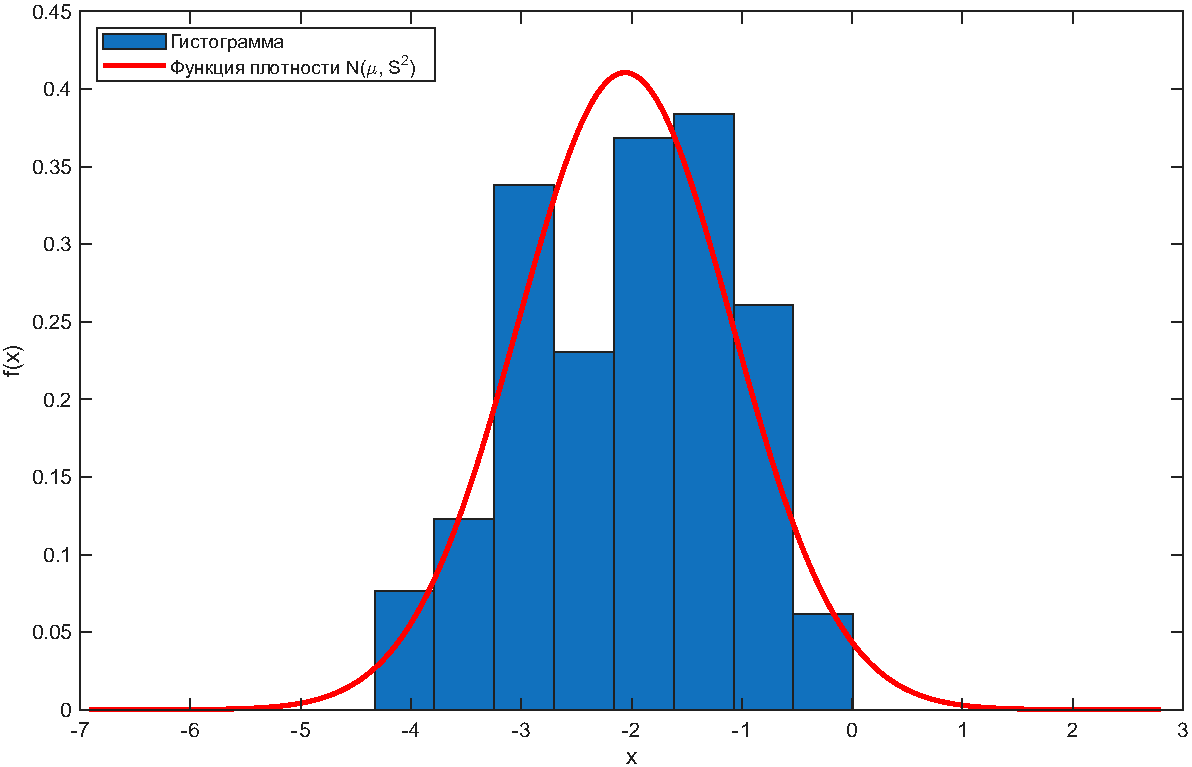
\includegraphics[scale=0.7]{./img/func_dp.pdf}
		\caption{Гистограмма и график функции плотности нормальной случайной величины}
		\label{image:graph1}
	}
\end{figure}

\clearpage

На рисунке \ref{image:graph2} представлены график эмпирической функции распределения и функции распределения нормальной случайной величины с математическим ожиданием $\hat\mu$ и дисперсией $S^2$.
\begin{figure}[h]
	\centering{
		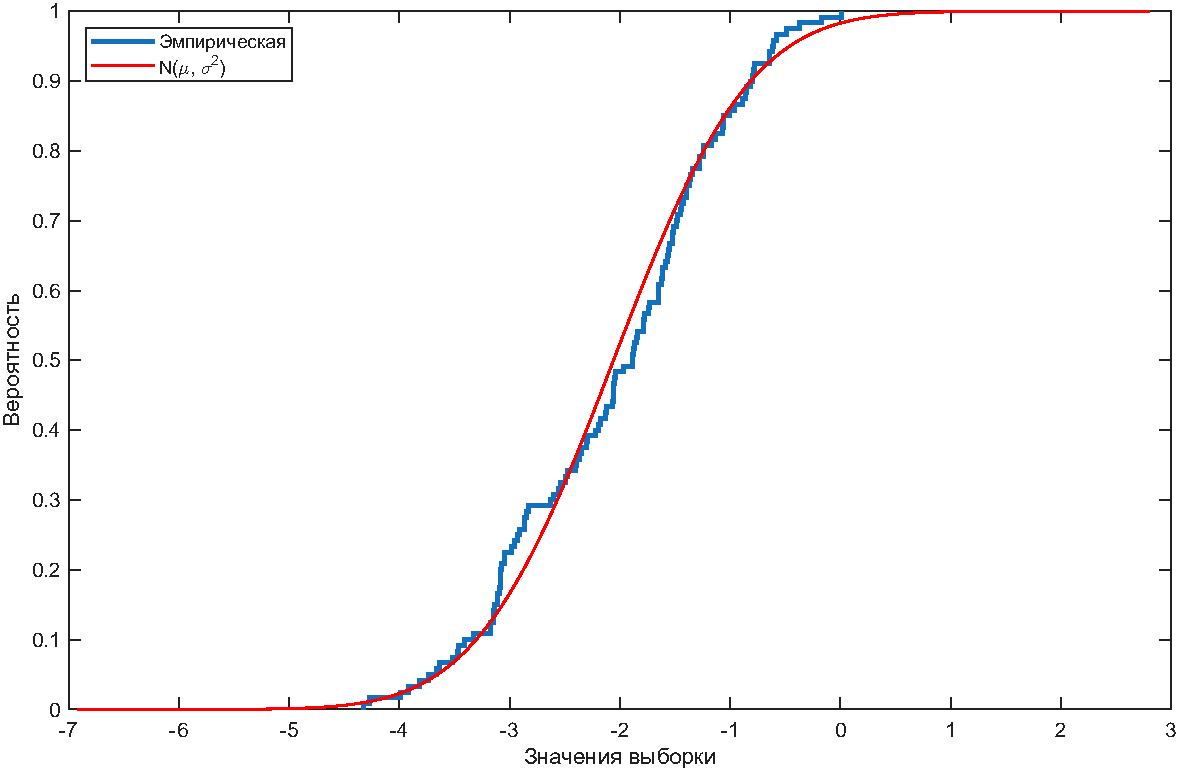
\includegraphics[scale=0.8]{./img/func_ep.pdf}
		\caption{Графики эмпирической функции распределения и функции распределения нормальной случайной величины}
		\label{image:graph2}
	}
\end{figure}
